\documentclass{article}
%\usepackage[margin=1in]{geometry}
\usepackage{graphicx} % Required for inserting images
\usepackage{hyperref}
\usepackage{amsmath}
\usepackage{titling}
\usepackage{enumitem}
\usepackage{makecell}
\usepackage{minted}
 \usepackage{url}
\renewcommand\maketitlehooka{\null\mbox{}\vfill}
\renewcommand\maketitlehookd{\vfill\null}

\begin{document}
\centering

\title{\Huge Intro Deep Learning Homework 1}

\author{ \huge
Jaskin Kabir \\
\Large Student Id: 801186717 \\
\Large \href{https://github.com/jaskinkabir/Intro_Deep_Learning/tree/master/HM1}{GitHub:}\\\url{https://github.com/jaskinkabir/Intro_Deep_Learning/tree/master/HM1}
}

\date{January 2025}

\begin{titlingpage}
\maketitle
\end{titlingpage}

\section{Problem 1: Multilayer Perceptrons For Image Classification}

\begin{enumerate}[label=1\alph*. ]
    \item \textit{Three Hidden Layers}
    
    Using three hidden layers, consisting of 64, 32, and 16
    neurons respectively, the model was trained for 20
    epochs. As seen in the curves graphed in Figure
    \ref{fig:loss_1a}, the training loss curve has not yet
    begun to converge to the optimal solution after just 20
    epochs. To fully train the model, more epochs would be
    required. There is also significant overfit, as
    indicated by the gap between the training and validation
    accuracy curves.
    
    \begin{figure}[h]
        \centering
        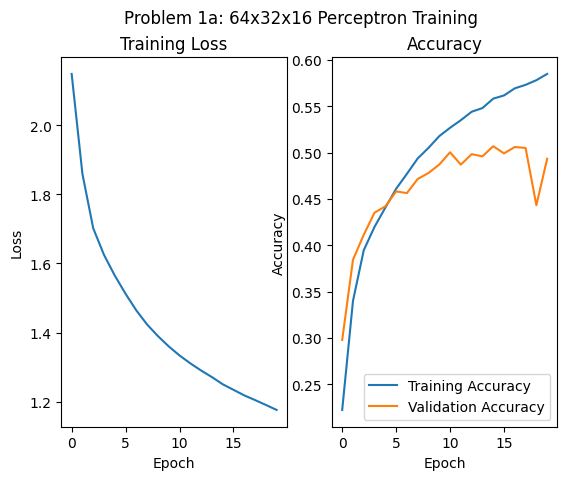
\includegraphics[width=0.5\textwidth]{images/loss_1a.png}
        \caption{Loss and Accuracy Curves for Three Hidden Layers}
        \label{fig:loss_1a}
    \end{figure} 
    The confusion matrix for this model can be seen in
    Figure \ref{fig:confusion_1a}.
    \begin{figure}[h]
        \centering
        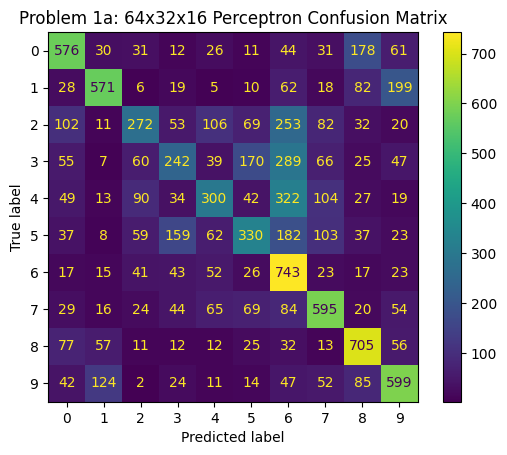
\includegraphics[width=0.5\textwidth]{images/conf_1a.png}
        \caption{Confusion Matrix for Three Hidden Layers}
        \label{fig:confusion_1a}
    \end{figure} 

    \newpage
    \item \textit{Five Hidden Layers}
    
    Using five hidden layers, consisting of 256, 128, 64,
    32, and 16 neurons respectively, the model was trained
    for 20 epochs. As seen in the curves graphed in Figure
    \ref{fig:loss_1b}, the model has not yet converged to
    the optimal solution after 20 epochs. There is also
    significant overfit, but not as pronounced as it is in
    the three hidden layer model.
    \begin{figure}[h]
        \centering
        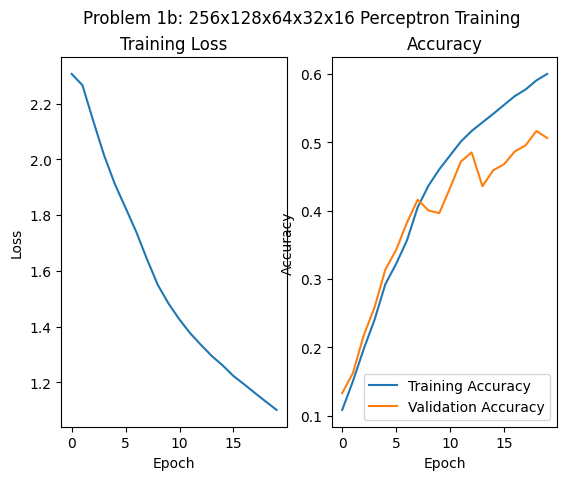
\includegraphics[width=0.5\textwidth]{images/loss_1b.png}
        \caption{Loss and Accuracy Curves for Five Hidden Layers}
        \label{fig:loss_1b}
    \end{figure}
    The confusion matrix for this model can be seen in
    Figure \ref{fig:confusion_1b}.
    \begin{figure}[h]
        \centering
        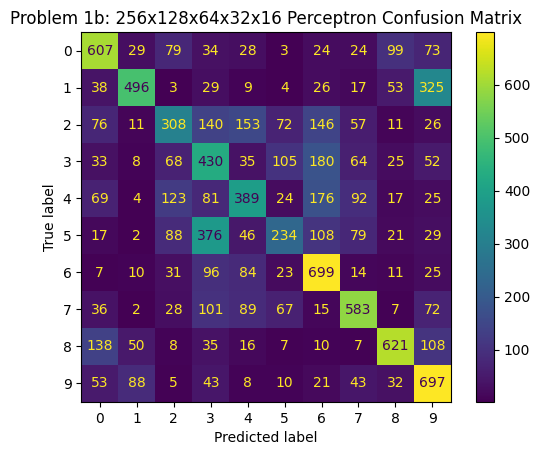
\includegraphics[width=0.5\textwidth]{images/conf_1b.png}
        \caption{Confusion Matrix for Five Hidden Layers}
        \label{fig:confusion_1b}
    \end{figure} 

\textbf{Comparison}

Table \ref{tab:comparison1} shows that the more complex
model performed better in every metric. However, even the
5-layer model was barely more accurate than a coin toss. The
models are likely underfit, as they have not yet converged
to the optimal solution. Additionally, the multilayer
perceptron is not the ideal paradigm for image
classification. A convolutional neural network would likely
outperform both of these models.
\begin{table}[h]
    \centering
    \begin{tabular}{|c|c|c|c|c|}
        \hline
        & \textbf{Accuracy} & \textbf{Precision} & \textbf{Recall} & \textbf{F1 Score} \\
        \hline
        \textbf{1a: 3-Layer Model} & 49.3 & 49.8 & 49.3 & 48.2 \\
        \hline
        \textbf{1b: 5-Layer Model} & 50.6 & 51.6 & 50.6 & 50.1 \\
        \hline
        \textbf{\Large$\Delta_{a \rightarrow b}$} & 2.59 & 3.37 & 2.59 & 3.69 \\
        \hline
    \end{tabular}
    \caption{Comparison of Evaluation Metrics}
    \label{tab:comparison1}
\end{table}
\end{enumerate}

\section{Problem 2: Housing Price Regression}
\begin{enumerate}[label=1\alph*. ]
    \item \textit{ML Perceptron Regressor}
    
    The housing dataset has several categorical features. In
    order to use this data to train the model, the
    categorical values like 'yes' or 'no' were converted to
    1 and 0 respectively. Using 3 layers, with each , the
    model was trained for 750 epochs. As seen in the curves
    graphed in Figure \ref{fig:loss_2a}, the model converged
    to its optimal solution. However, the gap between the
    training and validation losses indicates significant
    overfit.
    \begin{figure}[h]
        \centering
        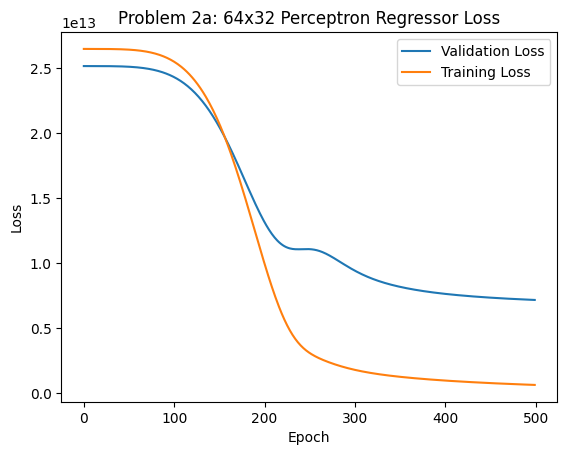
\includegraphics[width=0.5\textwidth]{images/loss_2a.png}
        \caption{Loss and Accuracy Curves for Perceptron Regressor}
        \label{fig:loss_2a}
    \end{figure}

    \item \textit{One-Hot Encoding}
    
    Instead of converting the categorical data to numerical
    values, one-hot encoding was used to convert each
    categorical feature into a number of binary features
    that correspond to each discrete value the feature could
    take on. This prevents the model from interpreting the
    categorical data as numerical and instead forces it to
    treat each category as a separate feature.
    
    The same model architecture was used as in the previous
    section and the model was trained for the same number of
    epochs. The curves plotted in Figure \ref{fig:loss_2b}
    show that the model suffered from overfitting, but it
    was not as significant as the previous model.
    \begin{figure}[h]
        \centering
        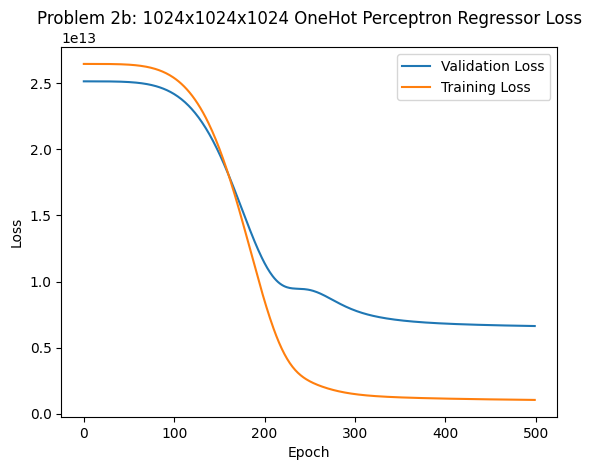
\includegraphics[width=0.5\textwidth]{images/loss_2b.png}
        \caption{Loss and Accuracy Curves for One-Hot Encoding}
        \label{fig:loss_2b}
    \end{figure}

    \item \textit{One-Hot Encoding With Increased
    Complexity} Using the same one-hot encoding method, a more complex model was
    trained on the dataset. This model used 512 neurons per layer, but had 8
    hidden layers. After training the model for 750 epochs, the validation loss
    curve began to increase due to overfit after about 150 epochs. Thus, the
    number of training epochs for this model was reduced to 150. As the curves
    plotted in Figure \ref{fig:loss_2c} show, the overfit was much less
    pronounced n this model, and the number of epochs was sufficient to reach an
    optimal solution.

    \begin{figure}[h]
        \centering
        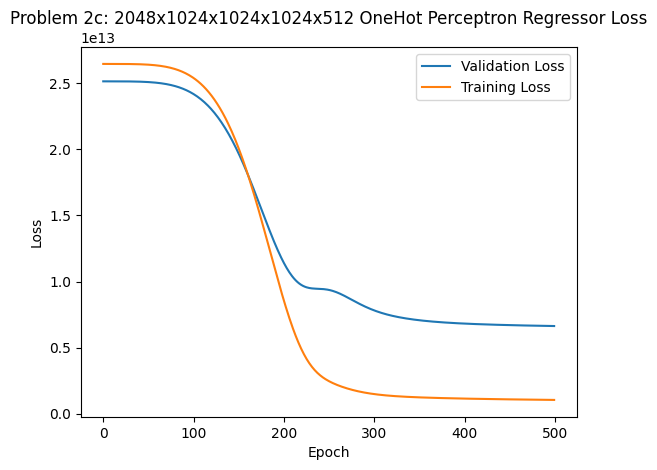
\includegraphics[width=0.5\textwidth]{images/loss_2c.png}
        \caption{Loss and Accuracy Curves for One-Hot Encoding With Increased Complexity}
        \label{fig:loss_2c}
    \end{figure}

    \newpage
    \textbf{Comparison}

    Table \ref{tab:comparison2} shows the root mean square and mean absolute
    losses for each of the three regressor models discussed thus far.
    Additionally, the table includes the percent difference between each pair of
    metrics. From the difference in mean absolute error, it is clear that the one-hot encoding only slightly
    improved the overall performance of the model when compared to the integer encoding. However, the higher
    improvement in RMS error indicates the model tended to make fewer large
    errors. The increased complexity of the third model greatly improved its
    performance compared to both of the previously explored models, however. The
    increased complexity allowed the model to learn more about the training
    data, and it was by far the best performing model.

    \begin{table}[h]
        \centering
        \begin{tabular}{|c|c|c|}
            \hline
             & \textbf{RMS Error} & \textbf{MAE} \\
            \hline
            \textbf{2a: Integer Encoding} & $2.62 \times 10^{6}$ & $1.98 \times 10^{6}$  \\
            \hline
            \textbf{2b: One-Hot Encoding} & $2.56 \times 10^{6}$ & $1.96 \times 10^{6}$\\
            \hline
            \textbf{2c: Complex One-Hot Model} & $2.35 \times 10^{6}$ & $1.80 \times 10^{6}$\\
            \hline
            \textbf{\large $\Delta_{a \rightarrow b}$\%} & 2.63 & 0.65 \\
            \hline
            \textbf{\large $\Delta_{a \rightarrow c}$\%} & 10.58 & 8.48 \\
            \hline
            \textbf{\large $\Delta_{b \rightarrow c}$\%} & 8.17 & 7.88 \\
            \hline
        \end{tabular}
        \caption{Comparison of Evaluation Metrics}
        \label{tab:comparison2}
    \end{table}



\end{enumerate}

\end{document}